\begin{figure}[t!]
\centering
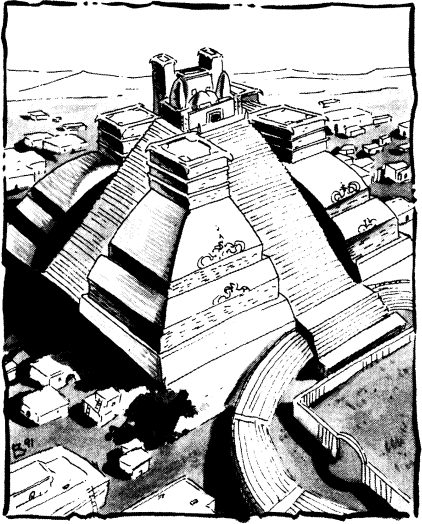
\includegraphics[width=\columnwidth]{images/draj-1.png}
\par\textit{\small\textcopyright Wizards of the Coast, 2020.}
\end{figure}

\City{Draj}
{15,000 (60\% humans, 15\% dwarves, 15\% elves, 5\% muls, 3\% half-elves, 2\% half-giants).}
{Wheat, rice, hemp, livestock, textiles, straw mats, pottery.}
{Common, Dwarven, Elven, Draji.}
{
	Draj, situated on a vast mud flat east of Raam, was another warlike city-state before its sorcerer-king was killed by Rajaat during his brief escape in FY 10. Before the news could cause panic and social upheaval in the city, King Tectuktitlay's templars (called ``moon priests'') quickly took stock of the situation, trying to find some way to preserve immortal Draj. The templars knew they had no real power without the spells granted by their sorcerer-king, so the supreme moon priests approached the most powerful masters of King Tectuktitlay's psionic academy, the House of the Mind. After numerous secret meetings, a plan was hit upon: The rulership of Draj would pass on to King Tec's ``son,'' a young psionicist named Atzetuk.

	The masters of the Way altered the teenager's mind, making him believe he was actually the king's son. Then they instructed him on what to say to the city's masses to instill confidence. In reality, the templars and psionic masters would share rulership of the city, working behind the scenes while the populace looked upon young Atzetuk as their new god-king. The transition from one king to another was accomplished quite easily; order had never been a problem in Draj, as its citizens were enraptured with the theocracy and religious trappings Tectuktitlay had surrounded himself with. As such, it was an easy task for the templars to use these rituals to save the city and keep the government running smoothly.
}
{
	Draj's citizens dress in loose, bright-colored shirts and skirts. All citizens wear headdresses of some sort, usually a roll of cloth or giant-hair braids, though the wealthy go in for more elaborate designs. By law only warriors may wear more than a single feather.

	The war festivals and religious ceremonies dedicated to the twin moons of Athas are the focus of life in Draj. The people have lost a god-king they neither respected nor believed in, but have gained a new god-king that is both well liked and inspires faith and reverence. This has surprised the secret leaders of the city, though not to the point where they have grown concerned. If their plan to replace King Tectuktitlay has succeeded beyond their wildest dreams, so much the better. Life in Draj remains the same as always---only the name of the king has changed.

	The natural disasters of the west never reached Draj. Rumors of a Great Earthquake arrived with the passing traders, but not even the slightest tremor or quake disturbed the city. Draj was inundated by one of the first Tyr-storms, however. The mud fields flooded, ruining crops and killing more than a few Draj citizens before the rain stopped falling and the wind and lightning abated.

	It didn't take long for the templars to clean up in the wake of the storm or for King Atzetuk to assuage the fears of his citizens. He called for sacrifices to appease the elementals, and the people of Draj approved. Atzetuk sent his warriors out into the wilderness to find captives worthy of dying on Draj's great pyramid, and before the week had passed rivers of blood washed over the pyramid's stone steps. Because of the relative closeness of the Cerulean Storm and because the Tyr-storms often pass within sight of Draj as they sweep inland, the sacrifices have become a regular ritual. The citizens believe that the blood will keep the storms at bay-after all, that's what their king has told them.

	The problems in Raam have had an effect on Draj. The templars and psionic masters watch the unfolding events as omens of what could occur in Draj if the illusion they've woven around Atzetuk ever unravels. Plus, many refugees have fled Raam and sought sanctuary in Draj. Most of these expatriates found only death, either in the mud flats or atop the bloody pyramid at the heart of the city. At some point, these lost exiles will find a voice and shout their grievances-and perhaps the citizens of Draj will hear that shout. The secret leaders fear Draj's society will collapse if the people lose faith in King Atzetuk.

	Atzetuk himself poses another problem for Draj's secret leadership. Every day, the youth gains more and more confidence. His belief in his own divinity strengthens.

	Soon, the masters of the Way suspect, they will lose control of the youth. While they don't want Draj to be overcome by anarchy and violence, they also don't want to give up the authority they've gained since Tectuktitlay's death. If Atzetuk continues to assert himself, the masters of the Way and the moon priests might decide to remove the king they put in place. After all, they reason, Draj survived the death of one king. It will surely survive the death of a second.
}
{
\begin{figure*}[b!]
\centering
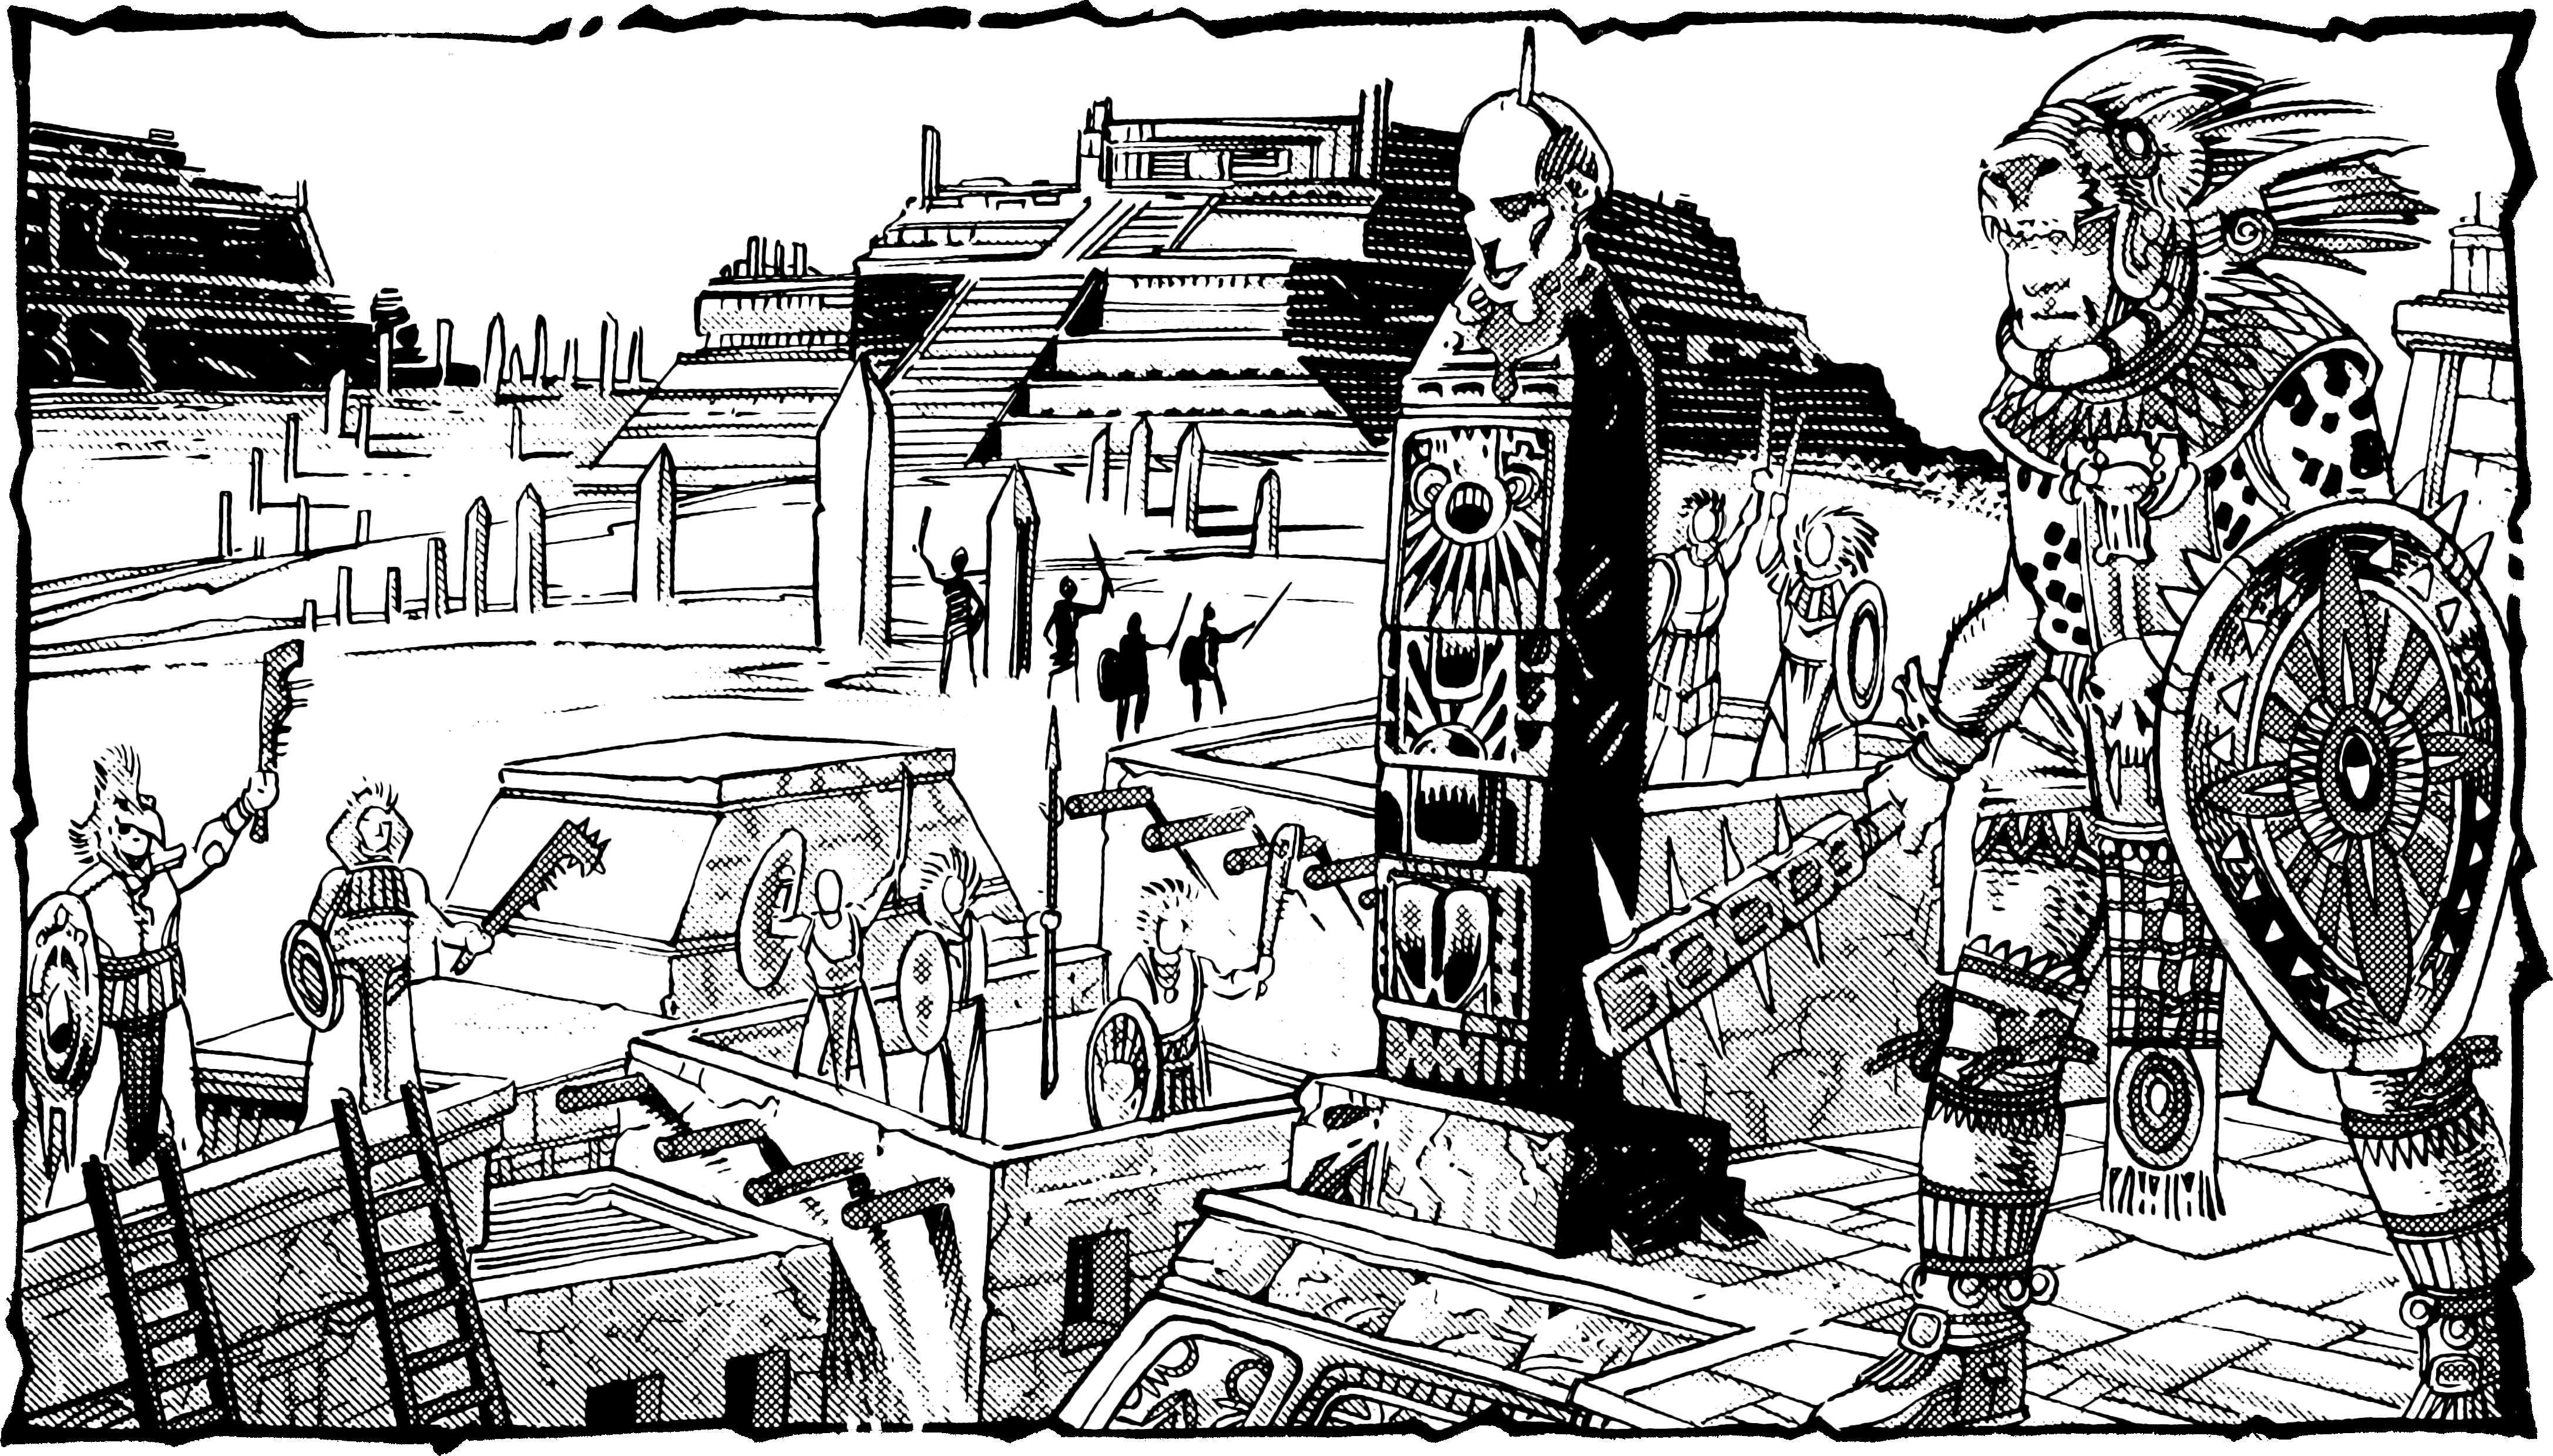
\includegraphics[width=\textwidth]{images/draj-2.png}
\par\textit{\small\textcopyright Wizards of the Coast, 2020.}
\end{figure*}

	Atzetuk (NG male human, telepath 6) apparently rules Draj, but he's nothing more than a figurehead who sits on the throne and carries on the practices and traditions of war set forth by King Tectuktitlay. The youth is paraded before his subjects every day and holds court in the Father and Master Temple. Although Atzetuk believes he's the legitimate heir to Tectuktitlay's throne and the true ruler of Draj, the business of government is managed by the moon priests and the masters of the House of the Mind. The templars have some power in this alliance, but the real leaders of the city are the masters of the Way, who bow to the commands of old lxtabai the Blind (LN male human, egoist 12). It's in everyone's interest to maintain this illusion. Without the young god-king, the nobles and free citizens would rebel against the rule of templars and mindbenders.

	Draj's noble families participate in the governing of the city through special meetings held at tecpans. In these long buildings, noble elders gather to debate and resolve problems considered too ordinary and routine to concern the moon priests and the new god-king. The noble elders are all great warriors. They will follow Atzetuk for as long as the warrior traditions and ceremonies are upheld.
}
{
	\textbf{Knights}: There are a number of knightly orders that are part of the Draji society. The two most important are the eagle knights and the jaguar knights. The eagle knights are among the most brutal and fanatical Draji warriors and rank second behind only the jaguar knights. The jaguar knights are the finest warriors of Draj. They undergo intense training to conquer their fear and strike fear in their opponents.

	\textbf{House Tsalaxa}: The merchants of House Tsalaxa conduct most of the trade for the city of Draj. Tsalaxa is known for its ruthless practices, well suited for a warrior culture. These traders regularly engage in espionage and intrigue in order to secure valuable contracts and business opportunities. The new head of the House, Yarsha Tsalaxa (LN female human, aristocrat 2/rogue 15), has some private doubts about the legitimacy of Atzetuk's rulership. However, she's still trying to settle her own position as leader of House Tsalaxa in the wake of her grandfather Ydris' death, and she doesn't want to express her concerns without solid proof to back them up. In the meantime, she'll continue to aggressively control the merchant house and keep the trade routes active and open to benefit the city and fill her own coffers.

	\textbf{The Veiled Alliance}: Draj's Veiled Alliance is hampered by poor leadership and indecisiveness. The current leader, Chimali Zaachila (LG female human, preserver 5), pretends to be much more powerful than she really is. Her lack of ability and training makes her reluctant to launch any daring programs that might reveal her secret. As such, the Alliance has no spies in high places, no active programs designed to thwart the king and his templars, and no plans to accomplish anything of lasting importance. The Alliance in Draj does offer some assistance to visiting preservers, but has little else to make it much more than a secret club for wizards.
}
{
	\textbf{Break Shore (Village, 100)}: Break Shore is a trading village on the shore of the Silt Sea. Originally a client-village of Raam, the Draji gained control over the village during a war between the two city-states centuries ago, when gold was discovered in the nearby Mastyrial Mountains. The gold mine has been nearly depleted, though Draji templars still supervise bands of slaves struggling to uncover any little bit of precious metal remaining.

	\textbf{Bitter Well (Village, 100)}: Bitter Well is located on the shore of the Silt Sea. Originally built by dwarves the village's buildings are made of stone, and a grand well lies at the center of the village. The buildings are packed close together and canvas drapes are hung between them to provide shade. However, the drapes also create a closed environment and traps the smell of unwashed bodies in the streets.

	\textbf{Ket (Village, 500)}: The village of Ket is located on a small mud flat completely surrounded by an inland silt basin. The only way to access the village is along a mile-long causeway. The village maintains lucrative grain fields, which have maintained the village for years. With the renewed contact with the city-states of the North, Ket is becoming an important stop for caravans on the way north from Draj, bringing more prosperity the villagers.
}
{
	\textbf{Father and Master Temple}: More often known just as the Great Pyramid, the Father and Master Temple is a grand pyramid of stone and marble that is easily the largest building in Draj. The Great Pyramid houses administrative offices as well as the King's private quarters. Treasure rooms are rumored to fill the lower levels of the pyramid.

	\textbf{Fort Ebon}: Fort Ebon is a major supply point for all Tsalaxa's caravans traveling west from Draj. Located between Draj and Raam, all of the House's caravans that travel to the other city-states of the Tyr region stop at the fort.

	\textbf{Fort Firstwatch}: A merchant fort owned by House M'ke, Firstwatch is a supply point mid way between Raam and Draj. The fort defenders see frequent raids by elf nomads and mercenaries hired by rival houses, especially House Tsalaxa.

	\textbf{Fort Ral}: Fort Ral is a supply route on the road north from Ket. The fort was built on the ruins of an ancient pyramid. A contingent of soldiers from Draj, mostly archers, garrisons the fort. The soldiers patrol the road around the fort for raiders who often attack caravans traveling between Kurn and Draj. If threatened with an overwhelming hostile force, the soldiers retreat to the much more defensible Ket.

	\textbf{Flower War Field}: Located on a flat plain outside of the city, this field is used twice a year to hold the ``Flowery Wars.'' During the flowery wars, soldiers of Draj dress in elaborate regalia involving jaguar headdresses and feathers. Though considered training by the officers, the results of the battle bring glory to the winner, and exile or death to the loser.

	\textbf{The Palace of Gladiatorial Combat}: The Palace is a circular arena in which gladiator combat takes place. Spectator stands surround two-thirds of the arena, with the rest of the area taken up by the observation hall of the king of Draj. The eight storey tall observation hall towers over the rest of the arena and is covered by bas-reliefs depicting various scenes of Tectuktitlay victorious in battle. The former king of Draj is flanked by two jaguars in every image. The observation hall is used by the king, his templars, and their guests.

	\textbf{Royal Menagerie}: King Tectuktitlay maintained a large menagerie of captured beast from the wastes. Located near the royal jaguar breeding pits, Tectuktitlay kept a number of vicious predatory beasts in stout cages. The beasts of the royal menagerie are never used in the gladiator arena and are given excellent care by a department of the templarate.

	\textbf{Two Moon City}: Two Moon City is the walled administrative center of Draj. It houses the Father and Master Temple pyramid, the temples to Ral and Guthay, the House of the Mind, the Palace of Gladiatorial Combat and other important sites. The only entrance to Two Moon City is through the Jaguar Gate.
}
{
	\item A number of jaguars has escaped from the king's pens. The jaguars pose a threat to the ordinary citizens of Draj and must be recaptured. However, it is a punishable offense for anyone to harm one of the sacred jaguars, so they must be recaptured without any injury coming to them. Unknown to the templars, the jaguars were released by a druid who actively hinders all attempts to recapture the jaguars.
	\item Scandal rocks the city, when a young Draji named Inkarri declares that he is a son of Tectuktitlay. Inkarri appears to be one year older than Atzetuk and has the support of a small but influential group of templars. When a few nobles show support for Inkarri's claim, the rulers of Draj move quickly to crush him. Forces are sent against Inkarri and his followers who are holed up in a fortified clan compound.
	\item One of the PCs begins to court a Draji woman. Her brothers consider this a grave insult to their family's honor because the PC is a foreigner. Until the PC pays a suitable ``blood price'' decided by the clan's elders, her brothers will seek to kill both the PC and the woman to restore their family's honor. The PC can kill the brothers but will still have to pay the ``blood price'' to the clan elders to prevent any more unrest with the clan.
	\item More than the normal number of slaves has been disappearing from the fields. The mudflats that surround Draj have been infested with kluzds. The serpents prey on those slaves who come too close to the mudflats.
	\item A furious Tyr-storm strikes Draj, causing death and destruction. A mob of distraught citizens forms outside the Temple of Storms, blaming the priests of rain for the Tyr-storm. Many of the Temple's supporters flock to the scene to protect the temple from the mob. With neither side backing down, a full riot seems imminent. Templars and soldiers also arrive on the scene intent on restoring order.
	\item Chimali Zaachila, head of the Veiled Alliance, is always on the lookout for magic objects which she can use to simulate spell casting. When she learns that one of the PCs has such an item, she sends agents of the Veiled Alliance to steal the item and bring it to her. 
}